\documentclass[10pt]{article}
\usepackage{listings}
\usepackage{amsmath}
\usepackage{graphicx}
\usepackage{cases}
\usepackage{framed}
\usepackage{xcolor}
\graphicspath{{./img/}}
\usepackage[a4paper, margin=1in]{geometry}
\date{}
\newcommand{\norm}[1]{\left\lVert#1\right\rVert}
\begin{document}
\title{Log do Programa}
\author{}
\maketitle
\section*{Questão 1}
\section*{Propriedades da viga}
\begin{itemize}
\item Tipo: hollow
\item Largura: 1
\item Raio externo: 0.08
\item Raio interno: 0.06
\item Área: 0.00879646
\item Volume: 0.00879646
\item \(E\): 207000000000
\item \(G\): 79300000000
\item Limite de escoamento: 290000000000
\item \(I_{z}\): 2.19911e-05
\item \(I_{y}\): 2.19911e-05
\item \(I_{p}\): 4.39823e-05
\end{itemize}
\section*{Valores}
\begin{itemize}
\item Forças Verticais:
\begin{itemize}
\item Valor: 9328.53, Posição: 1
\item Valor: -14000, Posição: 0.6
\end{itemize}
\item Forças Horizontais:
\begin{itemize}
\item Valor: 5829.11, Posição: 1
\end{itemize}
\item Momentos:
\begin{itemize}
\end{itemize}
\item Torques:
\begin{itemize}
\item Valor: 5600, Posição: 0.6
\end{itemize}
\item Carregamentos:
\begin{itemize}
\item Função: \( 3100 x^{1} +  0 x^{0}\), Posição: \([0.04-0.4]\)\end{itemize}
\end{itemize}
\section*{Funções de Singularidade}
\begin{itemize}
\item Carregamentos, Forças Verticais e Momentos:
\begin{itemize}
\item \( 9328.53{\langle x-1 \rangle}^{-1} \) 
\item \( -14000{\langle x-0.6 \rangle}^{-1} \) 
\item \( 3100{\langle x-0.04 \rangle}^{1} \) 
\item \( -3100{\langle x-0.4 \rangle}^{1} \) 
\item \( -1116{\langle x-0.4 \rangle}^{0} \) 
\end{itemize}
\item Forças Horizontais:
\begin{itemize}
\item \( 5829.11{\langle x-1 \rangle}^{-1} \) 
\end{itemize}
\item Torques:
\begin{itemize}
\item \( -5600{\langle x-0.6 \rangle}^{-1} \) 
\end{itemize}
\end{itemize}
\section*{Equações}
\subsection*{Equação das forças verticais e momentos externos}
\[{\scriptstyle q(x) = M{\langle x-0 \rangle}^{-2} + Fy{\langle x-0 \rangle}^{-1} + 9328.53{\langle x-1 \rangle}^{-1} - 14000{\langle x-0.6 \rangle}^{-1} + 3100{\langle x-0.04 \rangle}^{1} - 3100{\langle x-0.4 \rangle}^{1} - 1116{\langle x-0.4 \rangle}^{0}
}\]\subsection*{Equação das forças cortantes}
\[{\scriptstyle V(x) = \int_{}^{} q(x) \,dx }\]\[{\scriptstyle V(x) = M{\langle x-0 \rangle}^{-1} + Fy{\langle x-0 \rangle}^{0} + 9328.53{\langle x-1 \rangle}^{0} - 14000{\langle x-0.6 \rangle}^{0} + 1550{\langle x-0.04 \rangle}^{2} - 1550{\langle x-0.4 \rangle}^{2} - 1116{\langle x-0.4 \rangle}^{1}
}\]\subsection*{Equação dos momentos internos}
\[{\scriptstyle M(x) = \int_{}^{} V(x) \,dx }\]\[{\scriptstyle M(x) = M{\langle x-0 \rangle}^{0} + Fy{\langle x-0 \rangle}^{1} + 9328.53{\langle x-1 \rangle}^{1} - 14000{\langle x-0.6 \rangle}^{1} + 516.667{\langle x-0.04 \rangle}^{3} - 516.667{\langle x-0.4 \rangle}^{3} - 558{\langle x-0.4 \rangle}^{2}
}\]\subsection*{Reações de apoio}
\[{\scriptstyle V(1^{+}) = M{\langle 1^{+}-0 \rangle}^{-1} + Fy{\langle 1^{+}-0 \rangle}^{0} + 9328.53{\langle 1^{+}-1 \rangle}^{0} - 14000{\langle 1^{+}-0.6 \rangle}^{0} + 1550{\langle 1^{+}-0.04 \rangle}^{2} - 1550{\langle 1^{+}-0.4 \rangle}^{2} - 1116{\langle 1^{+}-0.4 \rangle}^{1}
 = 0}\]\[{\scriptstyle V(1^{+}) = M \cdot 0 + Fy \cdot 1 + -4470.59  = 0}\]\[{\scriptstyle M(1^{+}) = M{\langle 1^{+}-0 \rangle}^{0} + Fy{\langle 1^{+}-0 \rangle}^{1} + 9328.53{\langle 1^{+}-1 \rangle}^{1} - 14000{\langle 1^{+}-0.6 \rangle}^{1} + 516.667{\langle 1^{+}-0.04 \rangle}^{3} - 516.667{\langle 1^{+}-0.4 \rangle}^{3} - 558{\langle 1^{+}-0.4 \rangle}^{2}
 = 0}\]\[{\scriptstyle M(1^{+}) = M \cdot 1 + Fy \cdot 1 + -5455.37  = 0}\]\[{\scriptstyle M = 984.775 }\]
\[{\scriptstyle Fy = 4470.59 }\]
\subsection*{Equação das forças horizontais}
\[{\scriptstyle f(x) = Fx{\langle x-0 \rangle}^{-1} + 5829.11{\langle x-1 \rangle}^{-1}
}\]\subsection*{Equação das forças normais}
\[{\scriptstyle N(x) = \int_{}^{} f(x) \,dx }\]\[{\scriptstyle N(x) = Fx{\langle x-0 \rangle}^{0} + 5829.11{\langle x-1 \rangle}^{0}
}\]\subsection*{Reações de apoio}
\[{\scriptstyle N(1^{+}) = Fx{\langle 1^{+}-0 \rangle}^{0} + 5829.11{\langle 1^{+}-1 \rangle}^{0}
 = 0}\]\[{\scriptstyle N(1^{+}) = Fx \cdot 1 + 5829.11  = 0}\]\[{\scriptstyle Fx = -5829.11 }\]
\subsection*{Equação dos torques}
\[{\scriptstyle t(x) = T{\langle x-0 \rangle}^{-1} + -5600{\langle x-0.6 \rangle}^{-1}
}\]\subsection*{Equação dos torques internos}
\[{\scriptstyle T(x) = \int_{}^{} t(x) \,dx }\]\[{\scriptstyle T(x) = T{\langle x-0 \rangle}^{0} + -5600{\langle x-0.6 \rangle}^{0}
}\]\subsection*{Reações de apoio}
\[{\scriptstyle T(1^{+}) = T{\langle 1^{+}-0 \rangle}^{0} + -5600{\langle 1^{+}-0.6 \rangle}^{0}
 = 0}\]\[{\scriptstyle T(1^{+}) = T \cdot 1 + -5600  = 0}\]\[{\scriptstyle T = 5600 }\]
\subsection{Inclinação}\[{\scriptstyle \theta (x) = \frac{1}{EI} \int_{}^{} M(x) \,dx }\]\[{\scriptscriptstyle \theta (0) = 0.00102462{\langle 0-1 \rangle}^{2} - 0.00153773{\langle 0-0.6 \rangle}^{2} + 2.83748e-05{\langle 0-0.04 \rangle}^{4} - 2.83748e-05{\langle 0-0.4 \rangle}^{4} - 4.08597e-05{\langle 0-0.4 \rangle}^{3} + 0.000216331{\langle 0-0 \rangle}^{1} + 0.00049104{\langle 0-0 \rangle}^{2} + C 1
 = 0 }\]\[{\scriptscriptstyle \theta (x) = 0.00102462{\langle x-1 \rangle}^{2} - 0.00153773{\langle x-0.6 \rangle}^{2} + 2.83748e-05{\langle x-0.04 \rangle}^{4} - 2.83748e-05{\langle x-0.4 \rangle}^{4} - 4.08597e-05{\langle x-0.4 \rangle}^{3} + 0.000216331{\langle x-0 \rangle}^{1} + 0.00049104{\langle x-0 \rangle}^{2}
}\]\subsection{Deflexão}\[{\scriptstyle v(x) = \int_{}^{} \theta (x) \,dx }\]\[{\scriptscriptstyle v(0) = 0.000341542{\langle 0-1 \rangle}^{3} - 0.000512576{\langle 0-0.6 \rangle}^{3} + 5.67495e-06{\langle 0-0.04 \rangle}^{5} - 5.67495e-06{\langle 0-0.4 \rangle}^{5} - 1.02149e-05{\langle 0-0.4 \rangle}^{4} + 0.000108166{\langle 0-0 \rangle}^{2} + 0.00016368{\langle 0-0 \rangle}^{3} + C 1
 = 0 }\]\[{\scriptscriptstyle v (x) = 0.000341542{\langle x-1 \rangle}^{3} - 0.000512576{\langle x-0.6 \rangle}^{3} + 5.67495e-06{\langle x-0.04 \rangle}^{5} - 5.67495e-06{\langle x-0.4 \rangle}^{5} - 1.02149e-05{\langle x-0.4 \rangle}^{4} + 0.000108166{\langle x-0 \rangle}^{2} + 0.00016368{\langle x-0 \rangle}^{3}
}\]\subsection{Alongamento}\[{\scriptstyle \Delta L (x) = \frac{1}{EA} \int_{}^{} N(x) \,dx }\]\[{\scriptscriptstyle \Delta L (0) = 3.20128e-06{\langle 0-1 \rangle}^{1} - 3.20128e-06{\langle 0-0 \rangle}^{1} + C 1
 = 0 }\]\[{\scriptscriptstyle \Delta L (x) = 3.20128e-06{\langle x-1 \rangle}^{1} - 3.20128e-06{\langle x-0 \rangle}^{1}
}\]\subsection{Torção}\[{\scriptstyle \phi (x) = \frac{1}{GI_{p}} \int_{}^{} M_{x}(x) \,dx }\]\[{\scriptscriptstyle \phi (0) = -0.0016056{\langle 0-0.6 \rangle}^{1} + 0.0016056{\langle 0-0 \rangle}^{1} + C 1
 = 0 }\]\[{\scriptscriptstyle \phi (x) = -0.0016056{\langle x-0.6 \rangle}^{1} + 0.0016056{\langle x-0 \rangle}^{1}
}\]\subsection*{Gráficos}
\begin{center}
    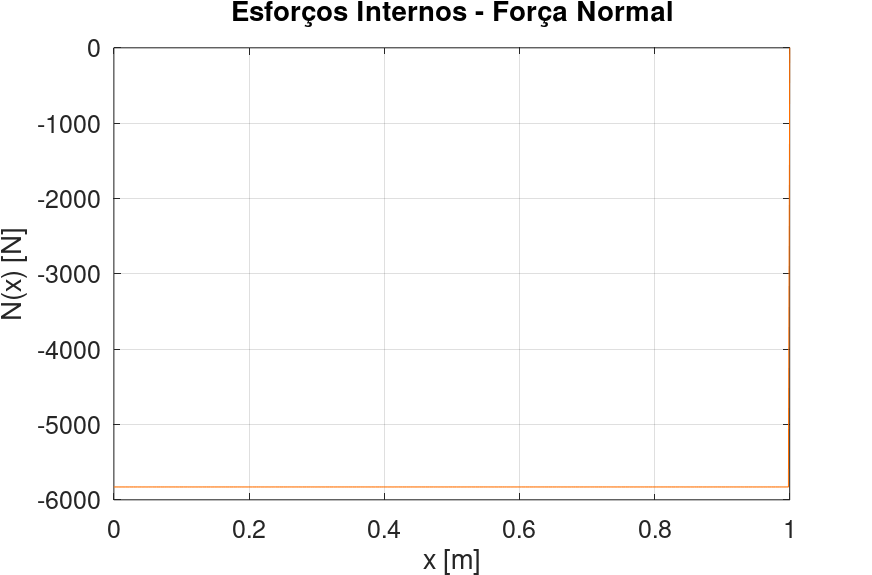
\includegraphics[scale=0.25]{figure1.png}
    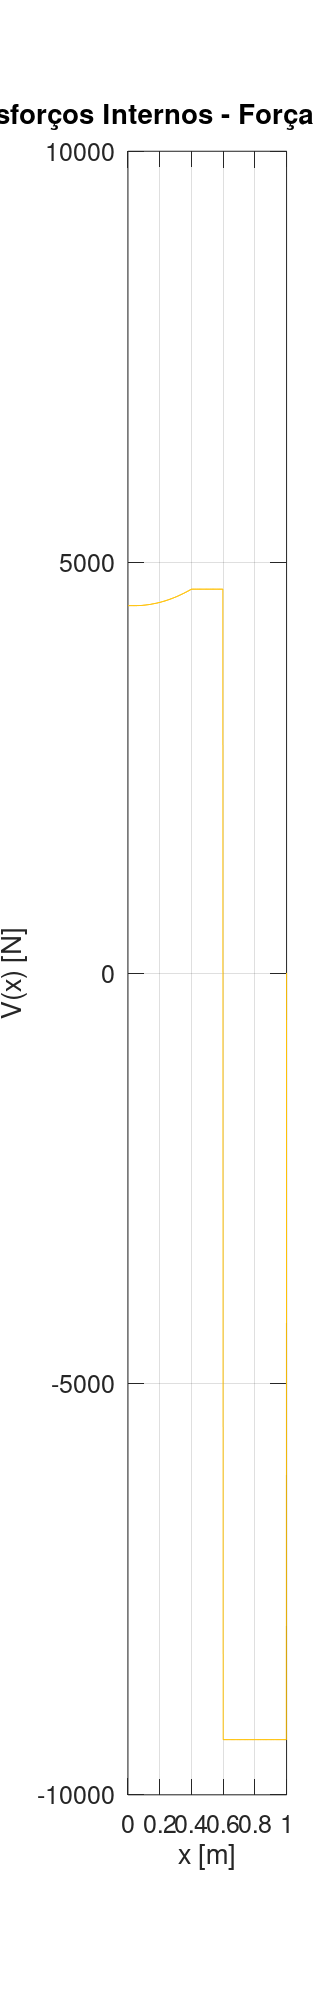
\includegraphics[scale=0.25]{figure2.png}
    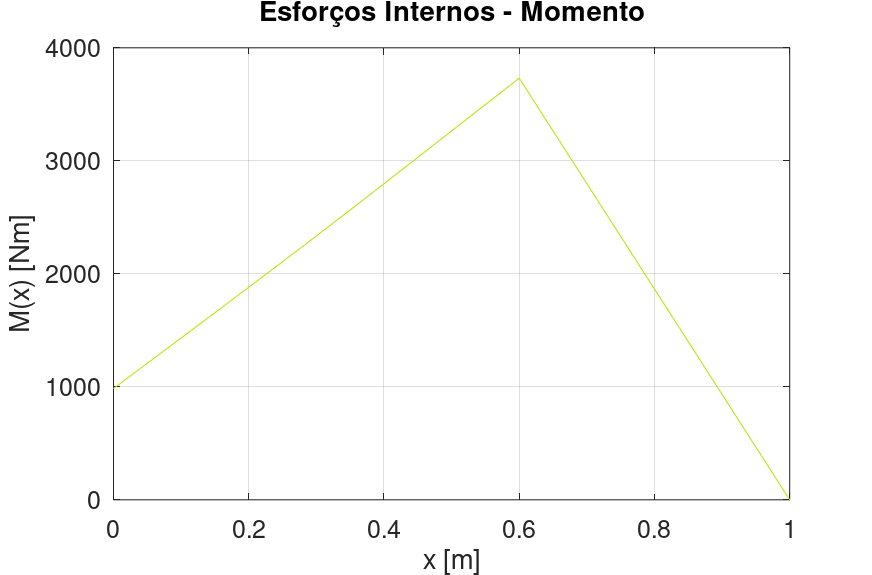
\includegraphics[scale=0.25]{figure3.png}
    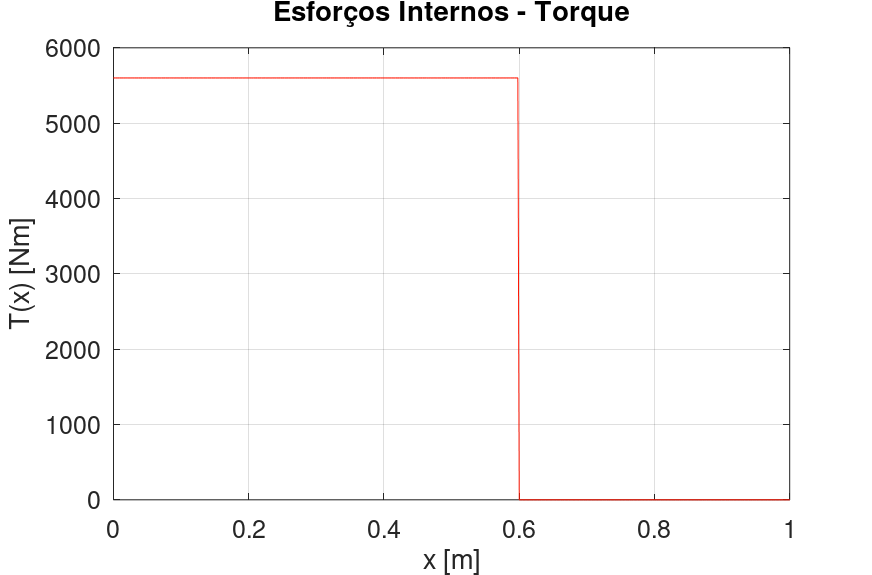
\includegraphics[scale=0.25]{figure4.png}
    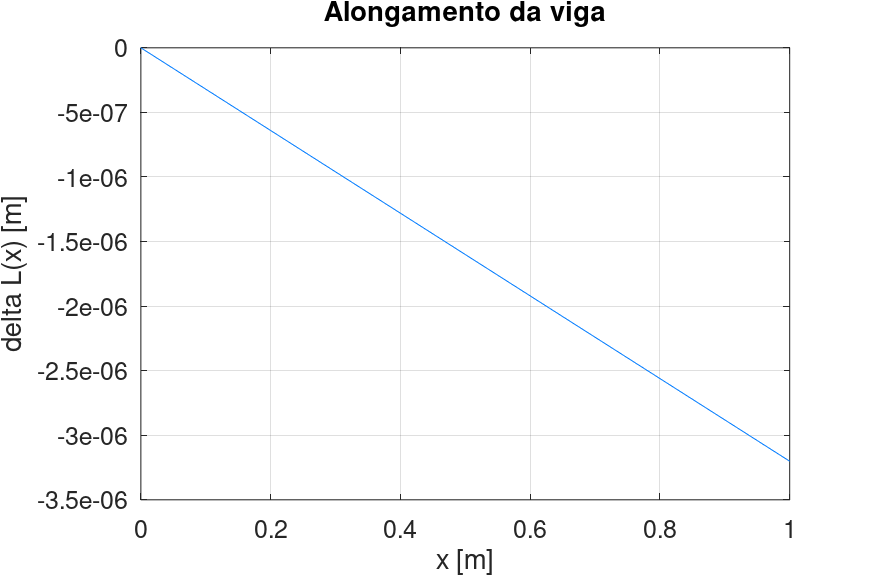
\includegraphics[scale=0.25]{figure5.png}
    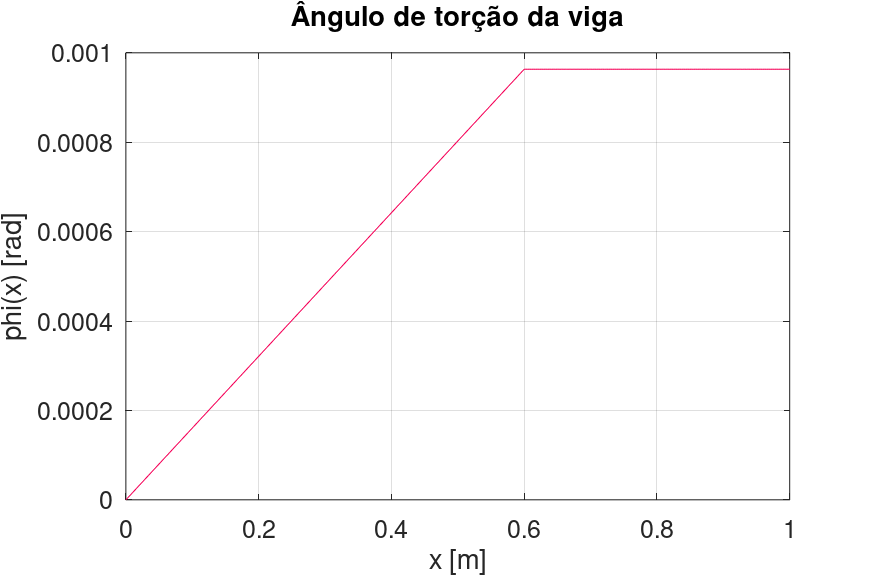
\includegraphics[scale=0.25]{figure6.png}
    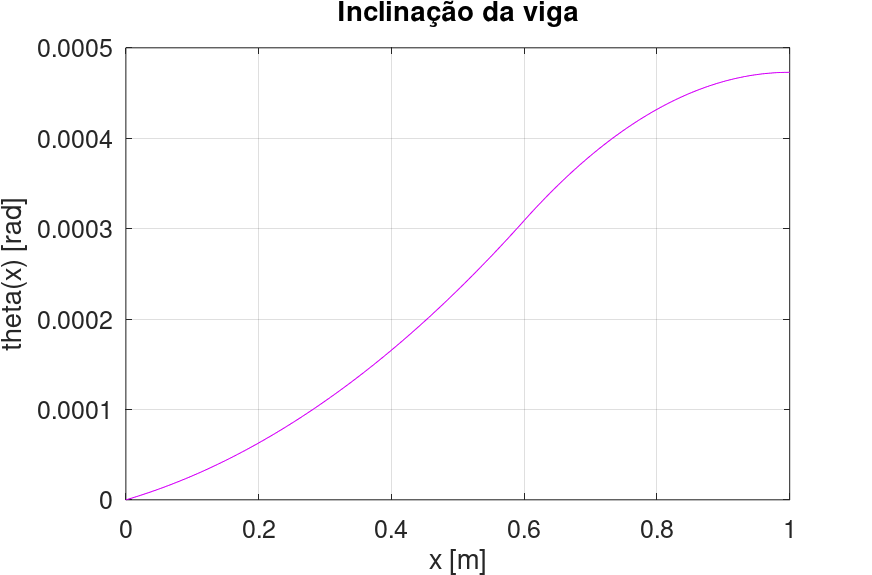
\includegraphics[scale=0.25]{figure7.png}
    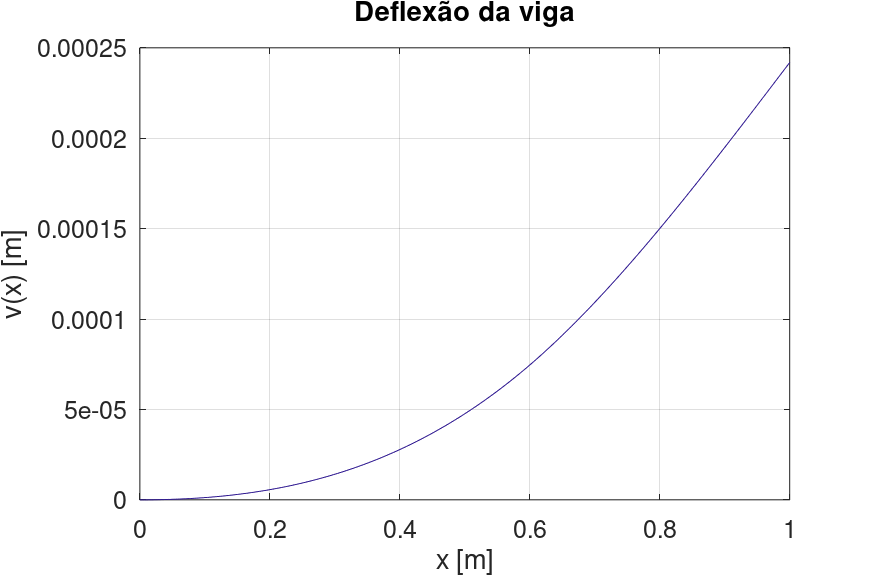
\includegraphics[scale=0.25]{figure8.png}
    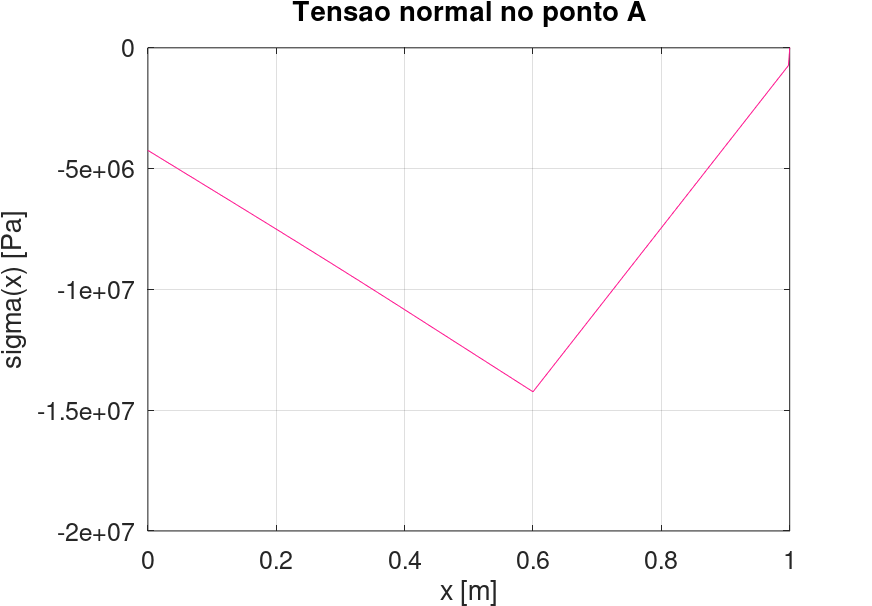
\includegraphics[scale=0.25]{figure9.png}
    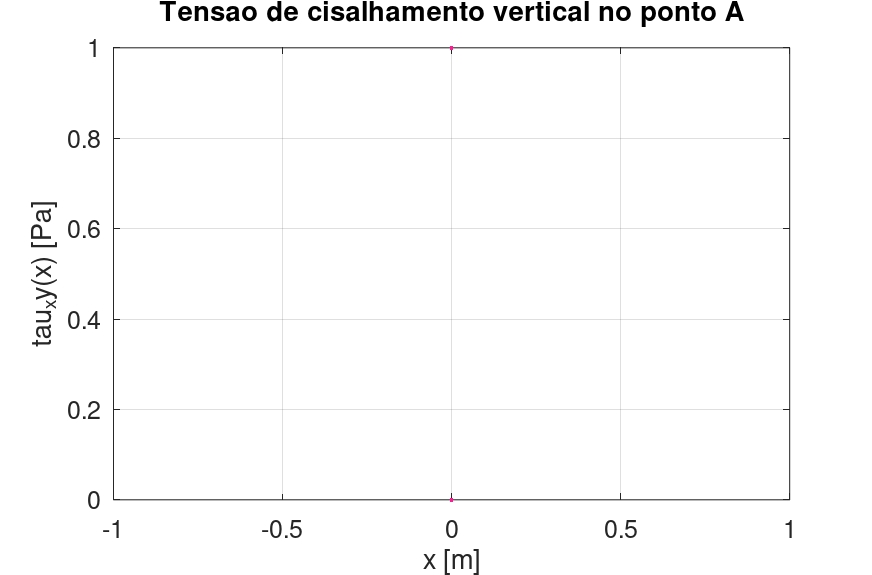
\includegraphics[scale=0.25]{figure10.png}
    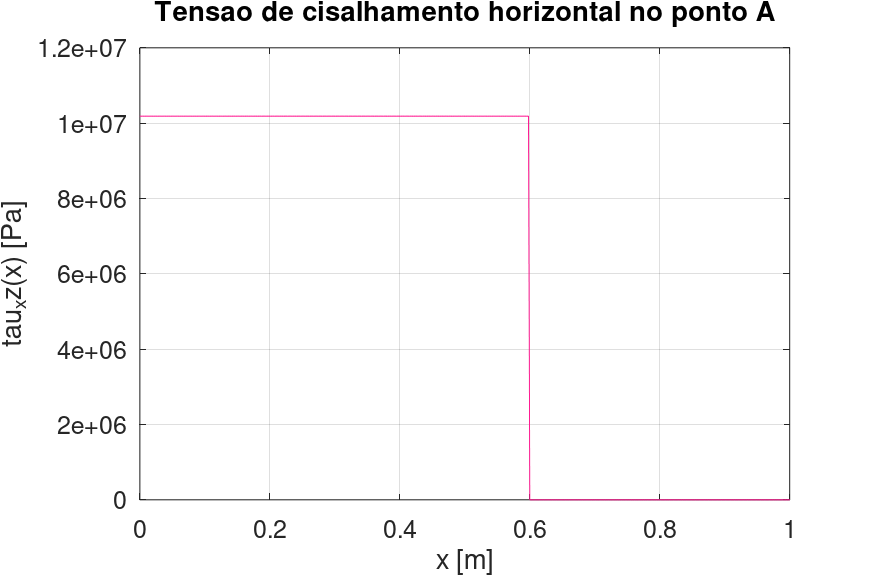
\includegraphics[scale=0.25]{figure11.png}
    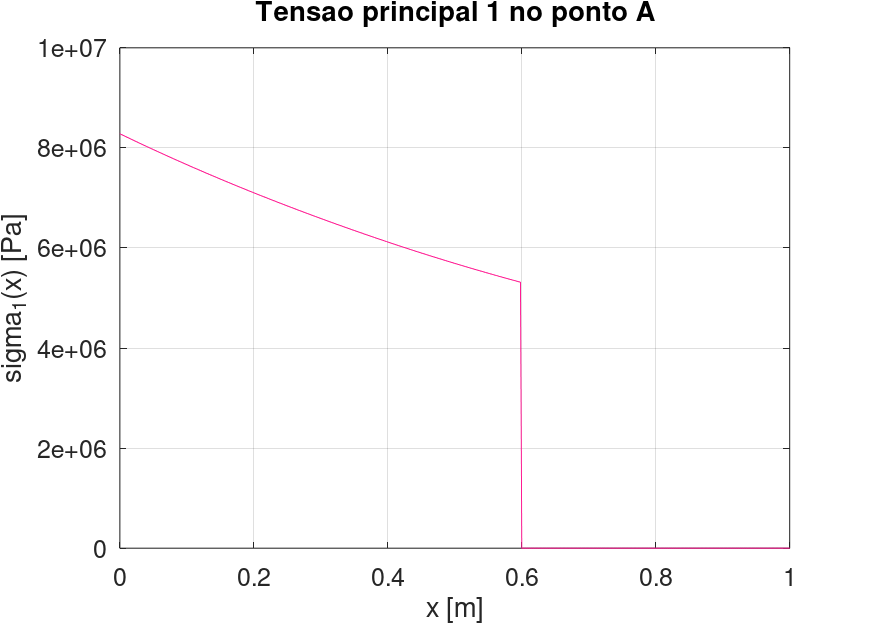
\includegraphics[scale=0.25]{figure12.png}
    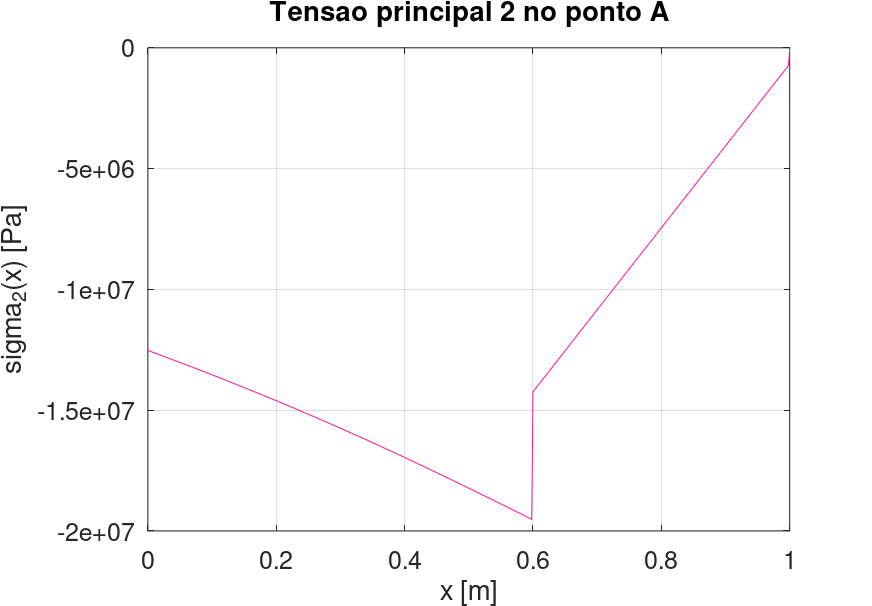
\includegraphics[scale=0.25]{figure13.png}
    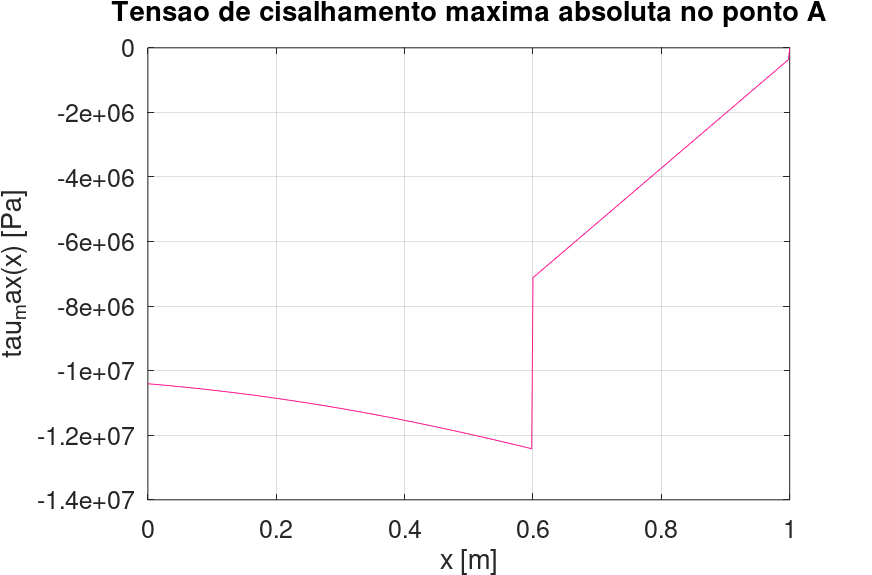
\includegraphics[scale=0.25]{figure14.png}
    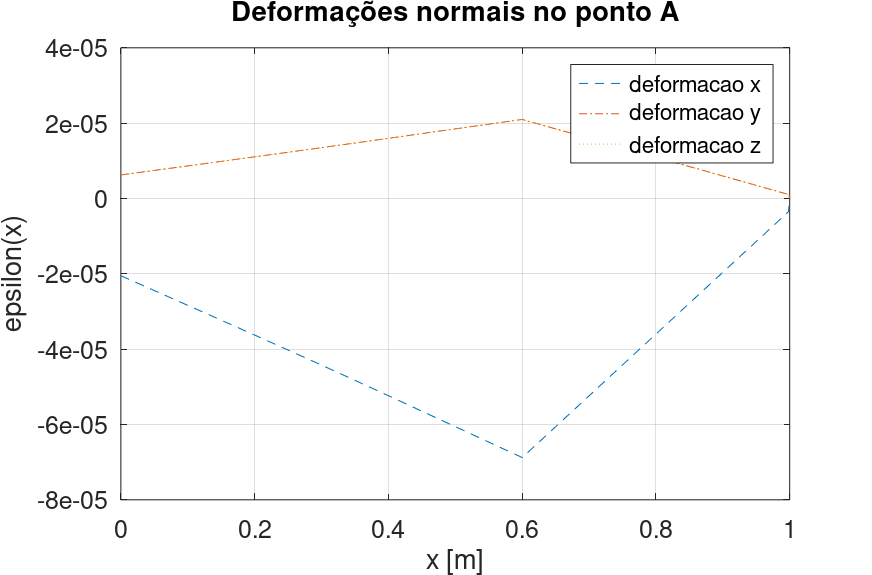
\includegraphics[scale=0.25]{figure15.png}
    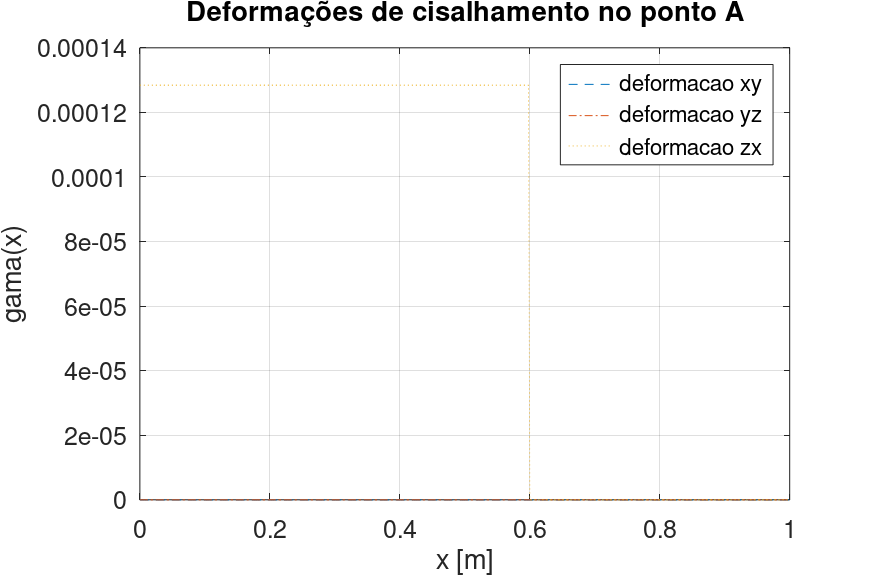
\includegraphics[scale=0.25]{figure16.png}
    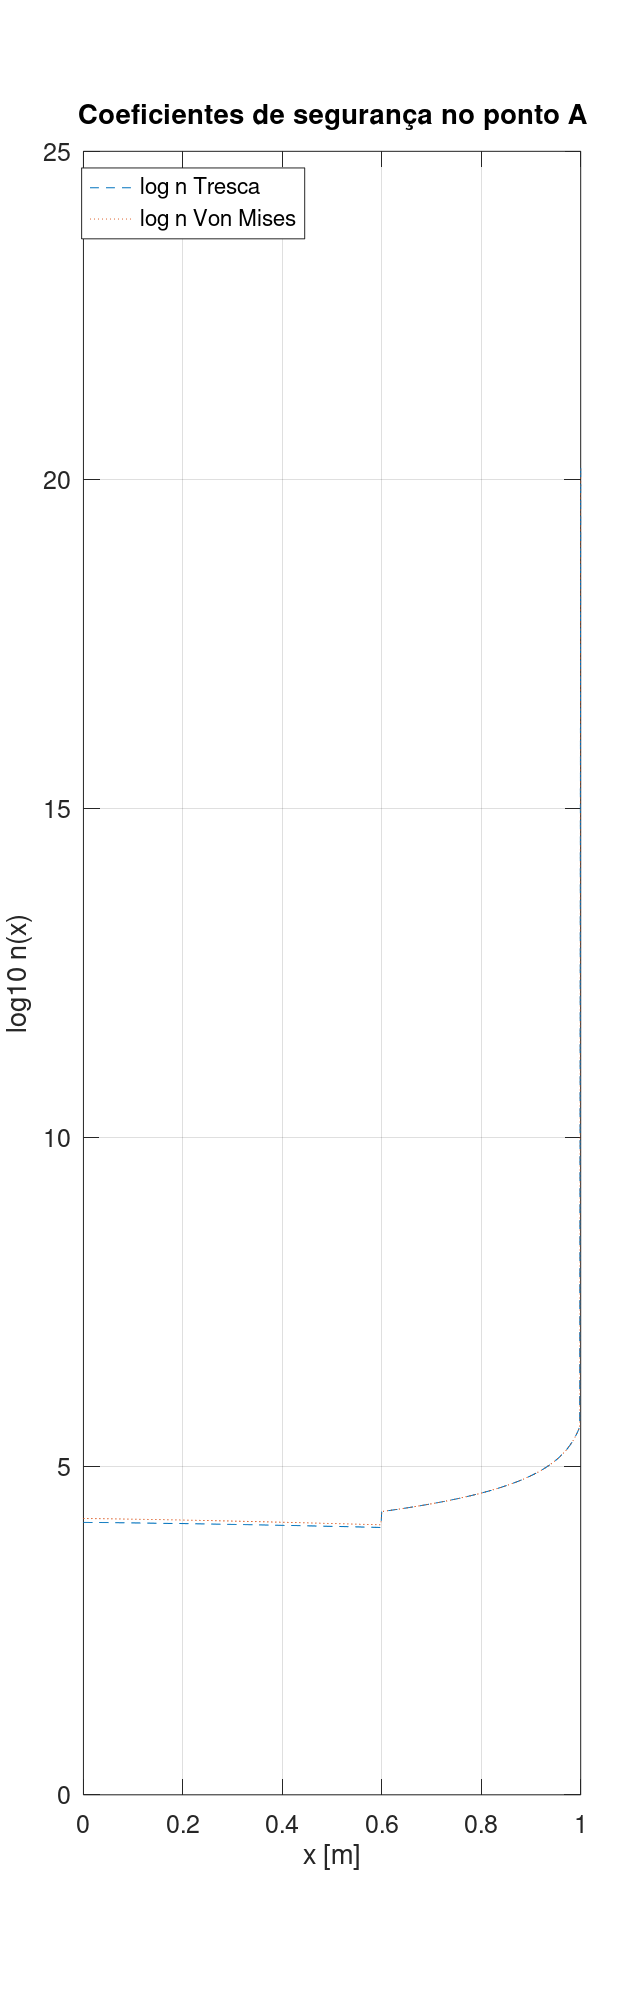
\includegraphics[scale=0.25]{figure17.png}
    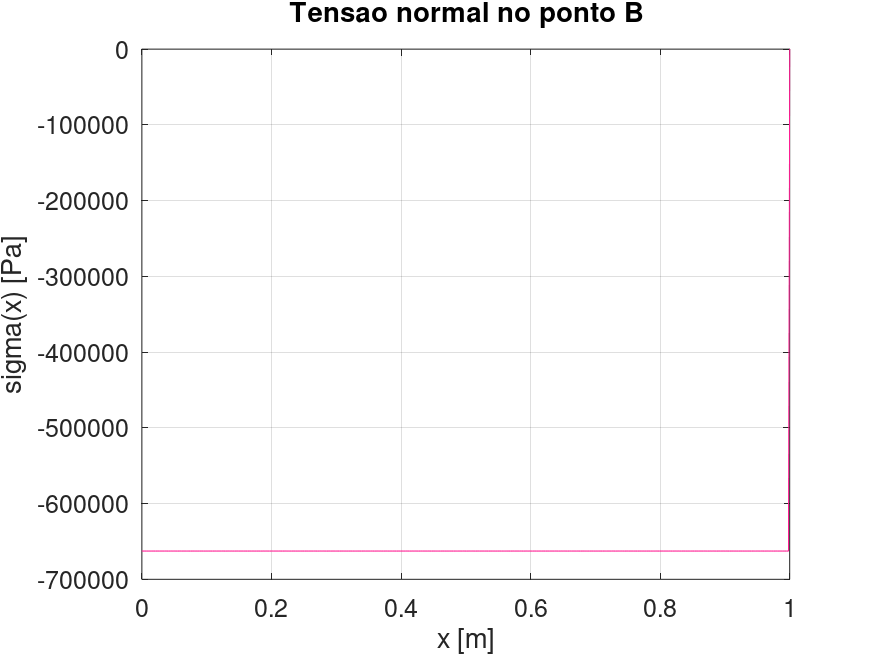
\includegraphics[scale=0.25]{figure18.png}
    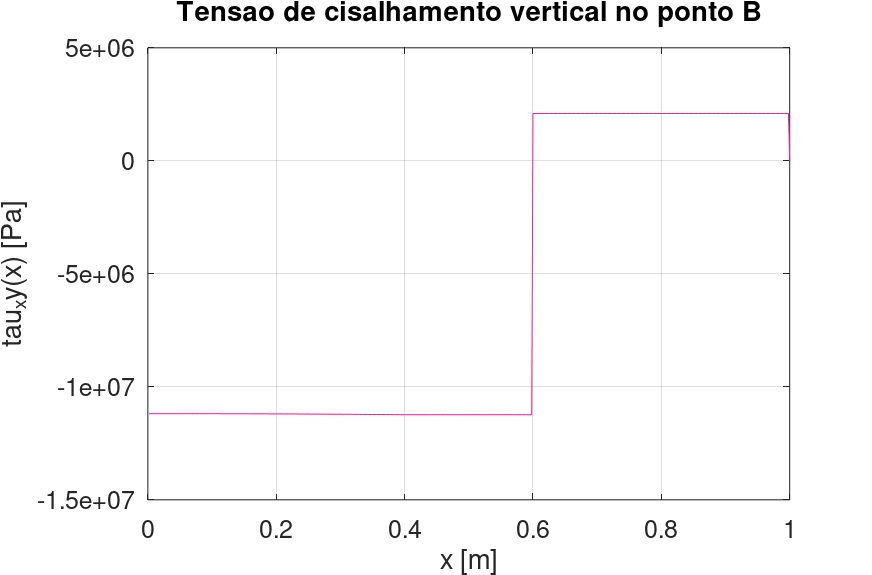
\includegraphics[scale=0.25]{figure19.png}
    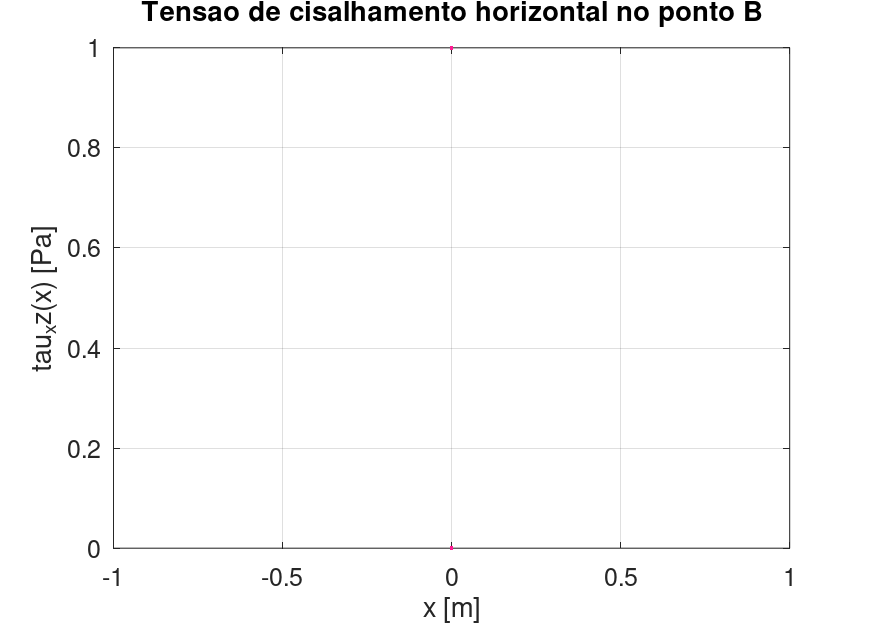
\includegraphics[scale=0.25]{figure20.png}
    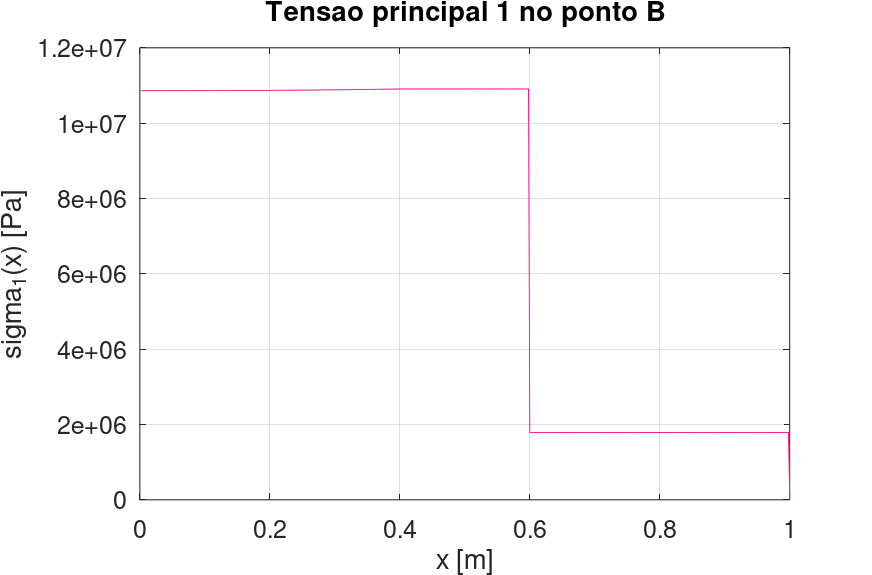
\includegraphics[scale=0.25]{figure21.png}
    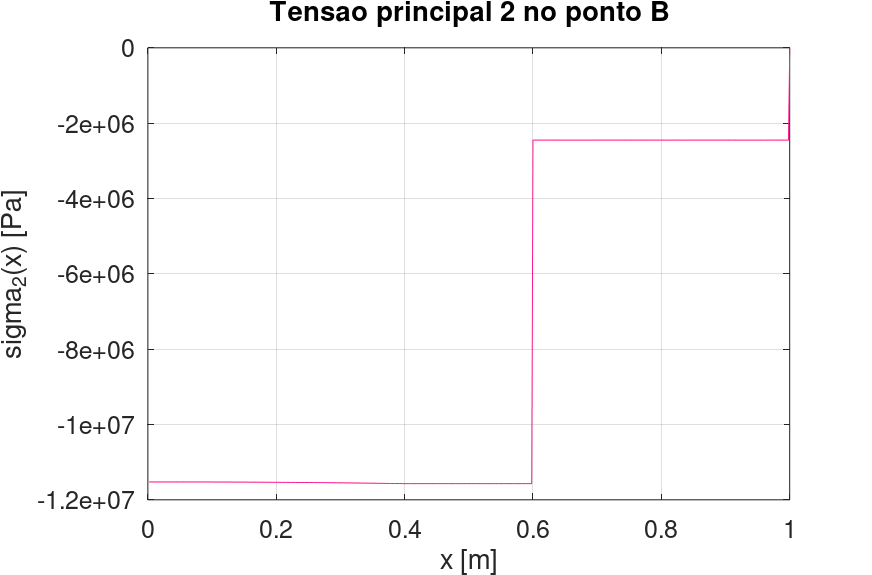
\includegraphics[scale=0.25]{figure22.png}
    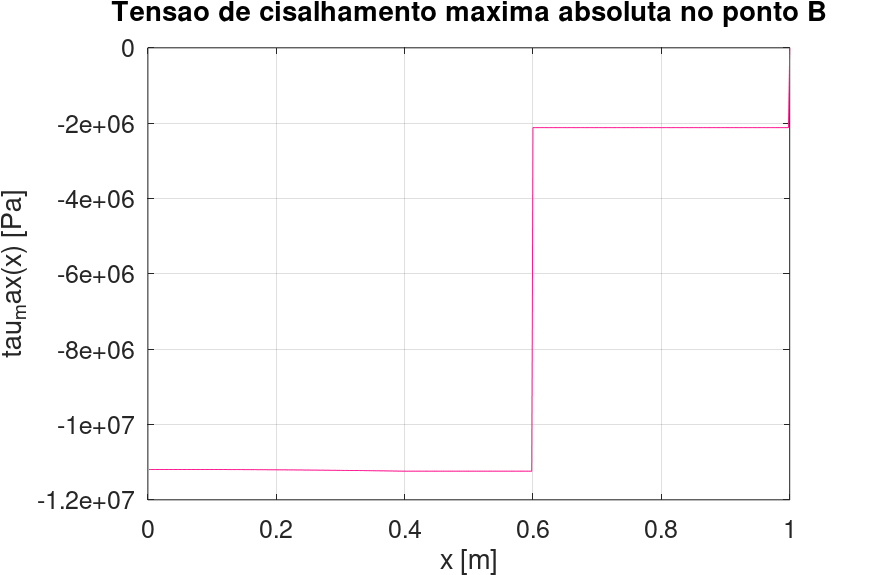
\includegraphics[scale=0.25]{figure23.png}
    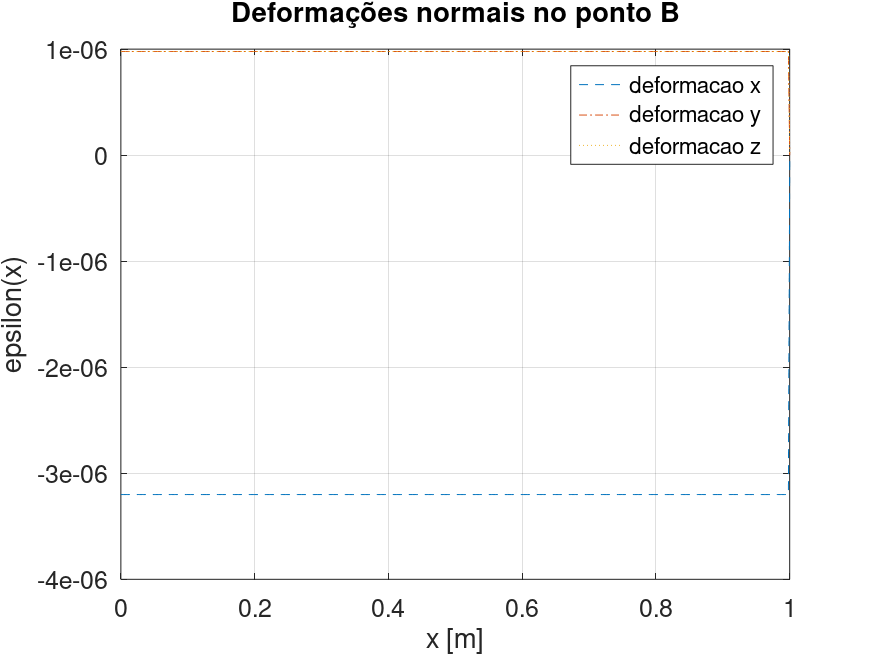
\includegraphics[scale=0.25]{figure24.png}
    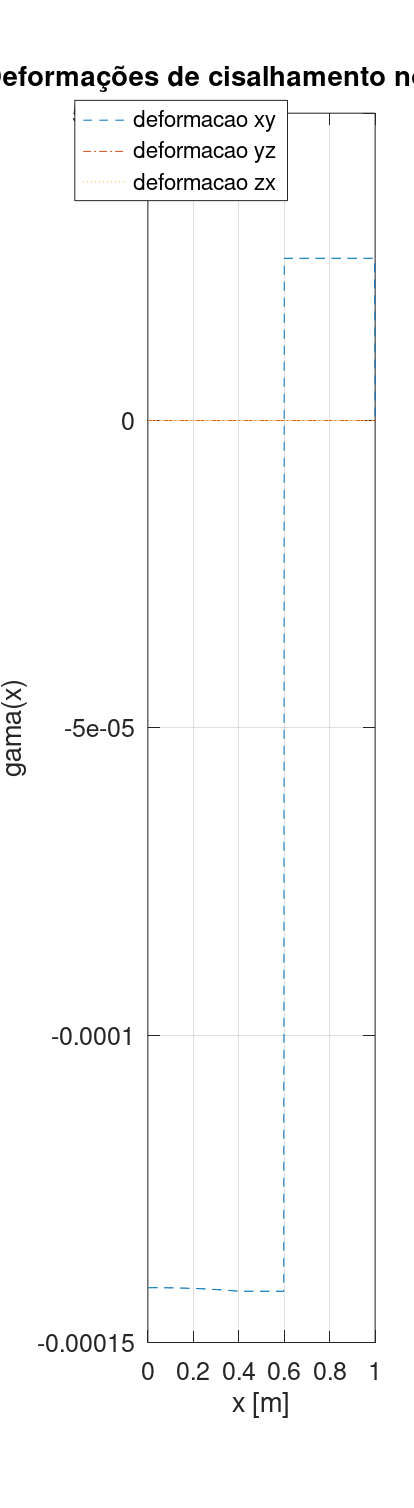
\includegraphics[scale=0.25]{figure25.png}
    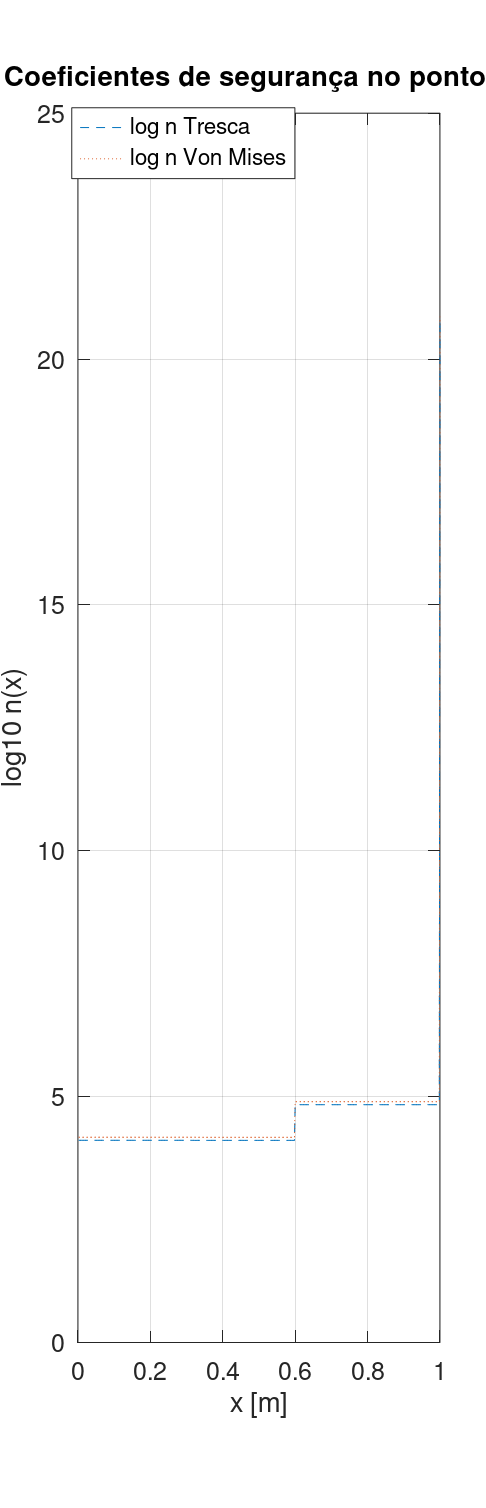
\includegraphics[scale=0.25]{figure26.png}
    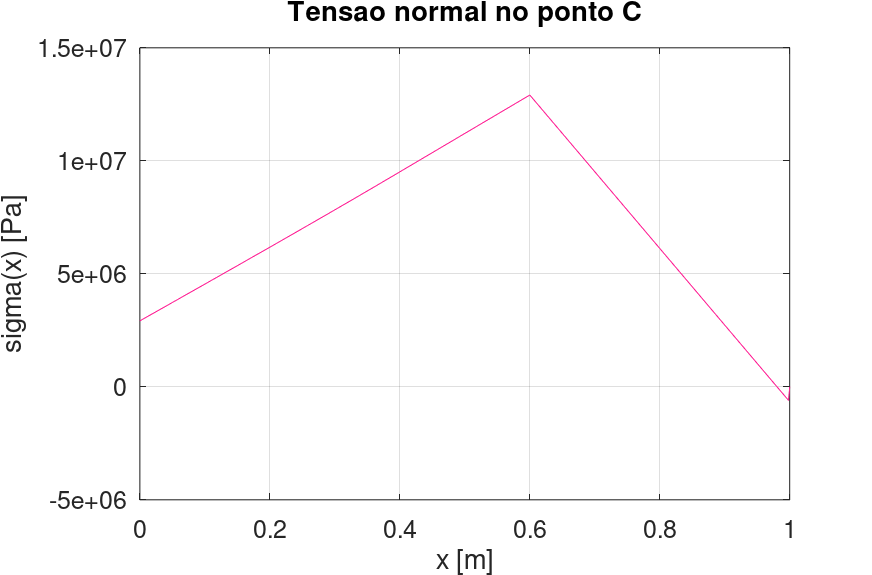
\includegraphics[scale=0.25]{figure27.png}
    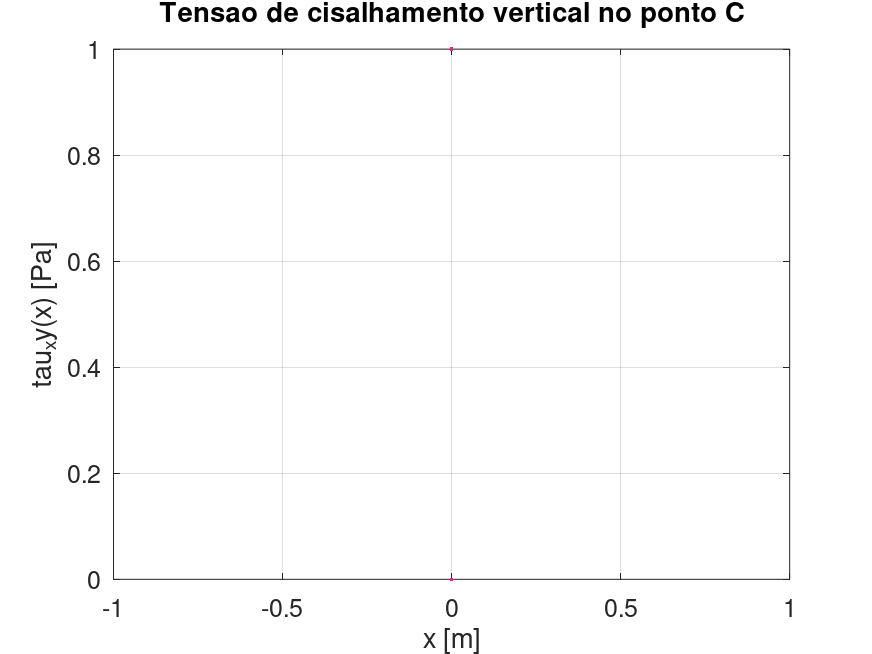
\includegraphics[scale=0.25]{figure28.png}
    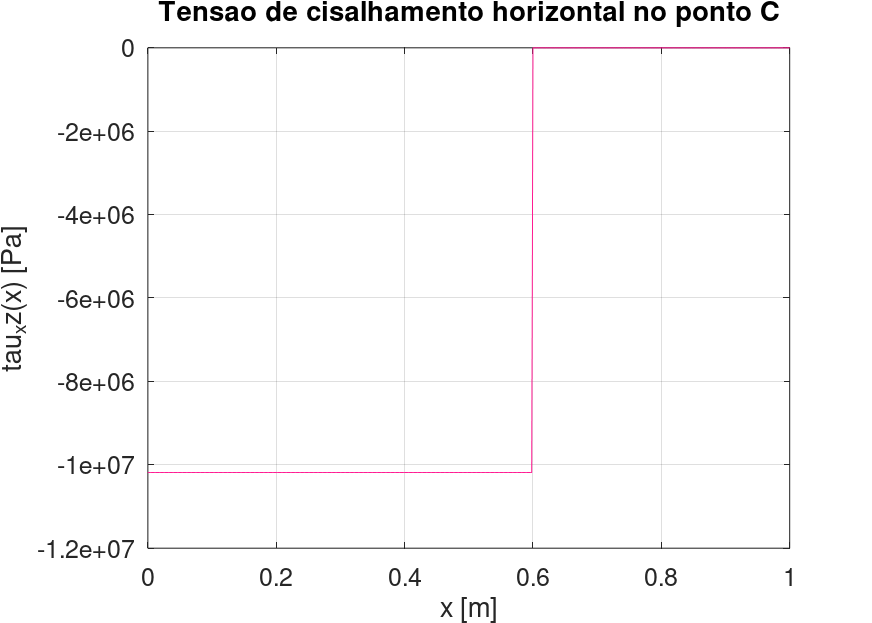
\includegraphics[scale=0.25]{figure29.png}
    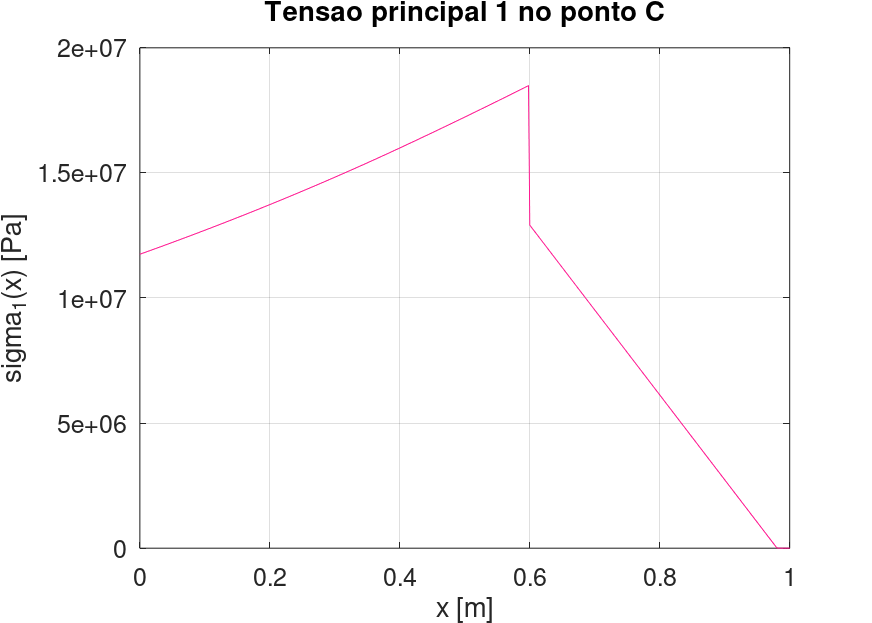
\includegraphics[scale=0.25]{figure30.png}
    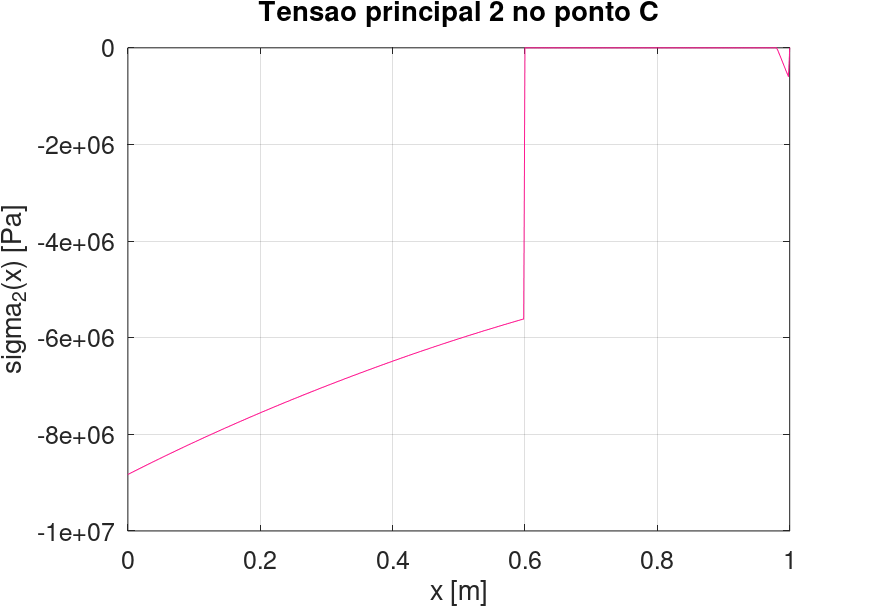
\includegraphics[scale=0.25]{figure31.png}
    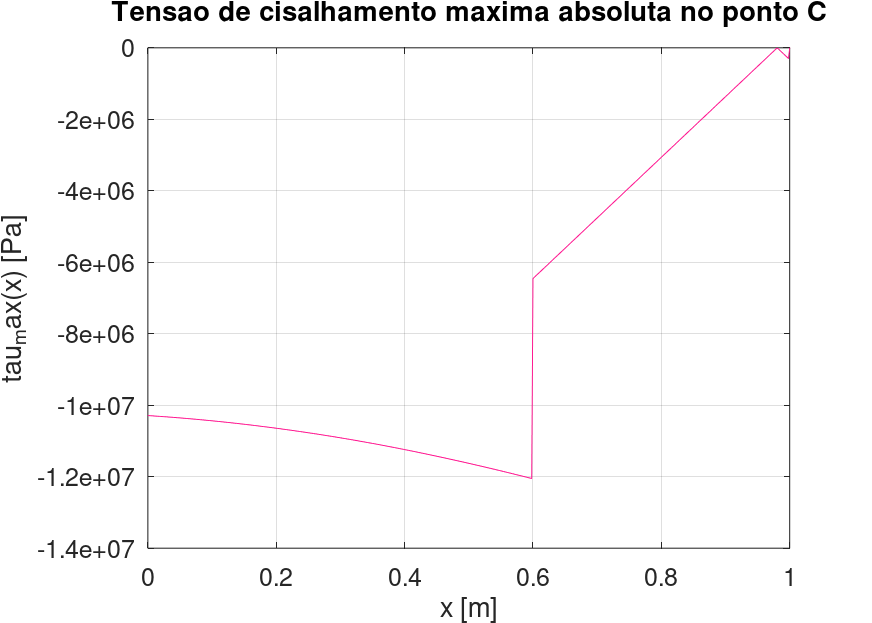
\includegraphics[scale=0.25]{figure32.png}
    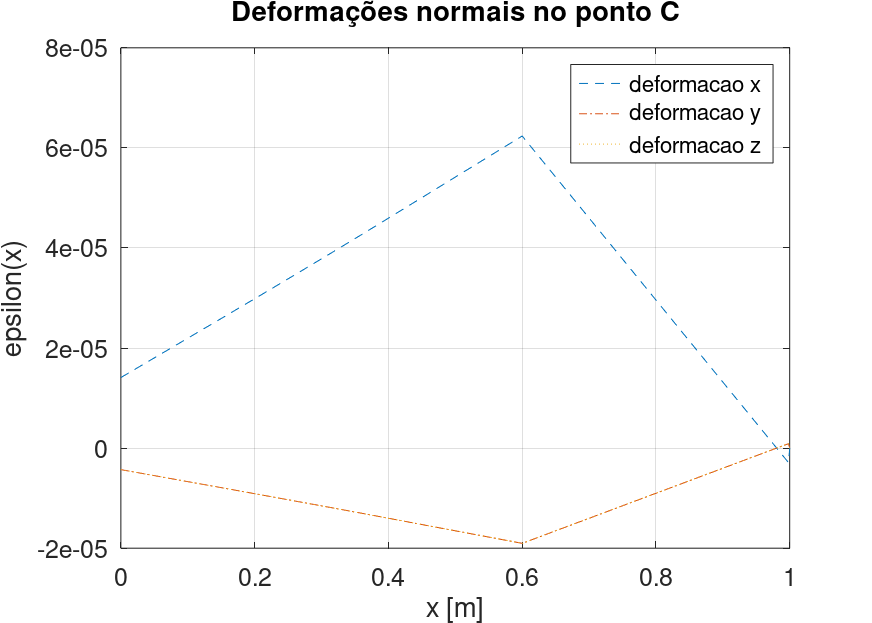
\includegraphics[scale=0.25]{figure33.png}
    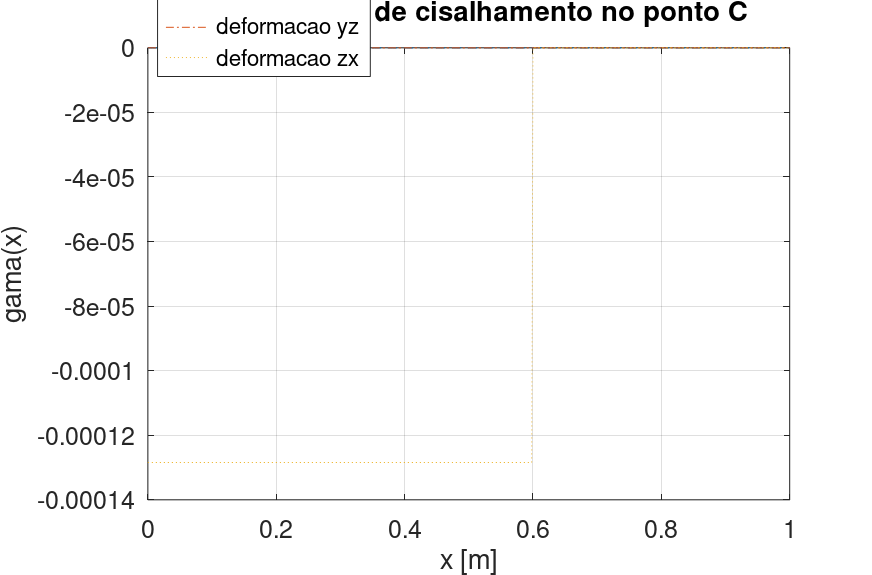
\includegraphics[scale=0.25]{figure34.png}
    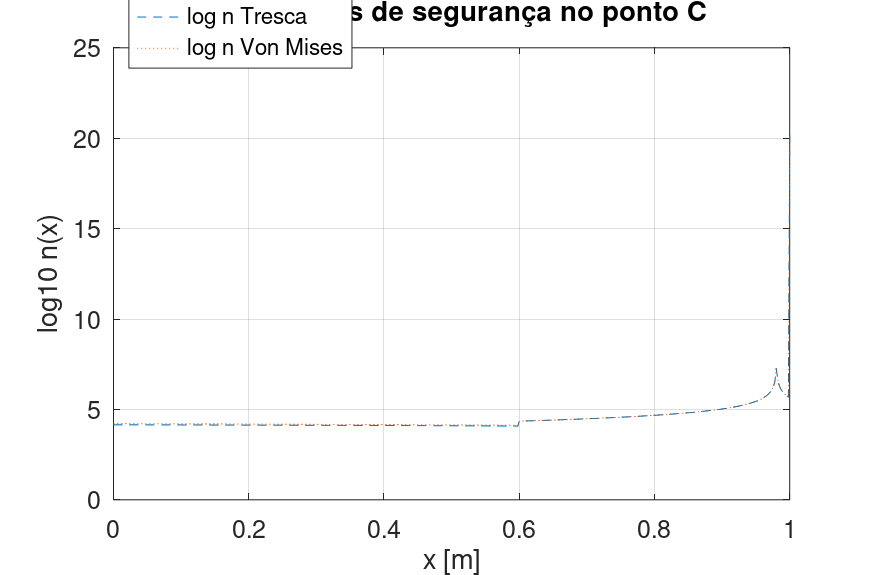
\includegraphics[scale=0.25]{figure35.png}
    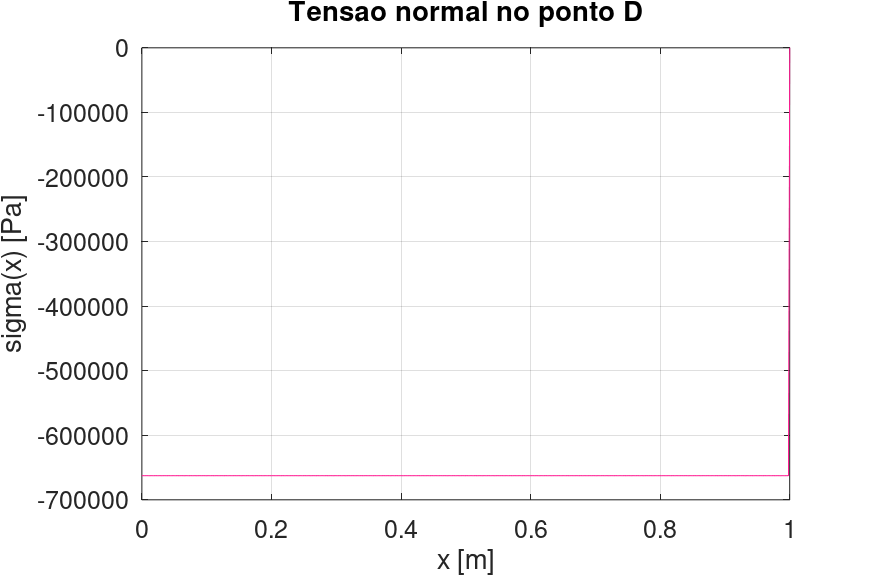
\includegraphics[scale=0.25]{figure36.png}
    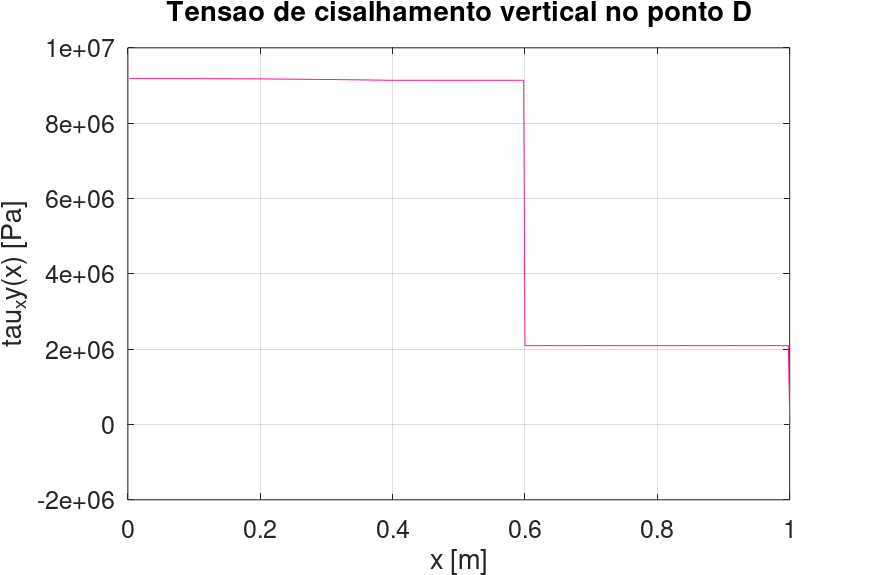
\includegraphics[scale=0.25]{figure37.png}
    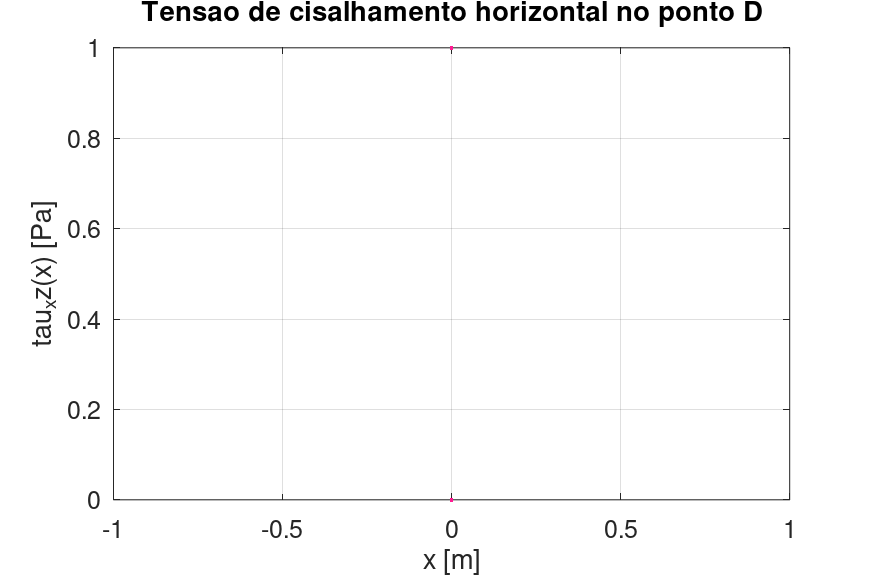
\includegraphics[scale=0.25]{figure38.png}
    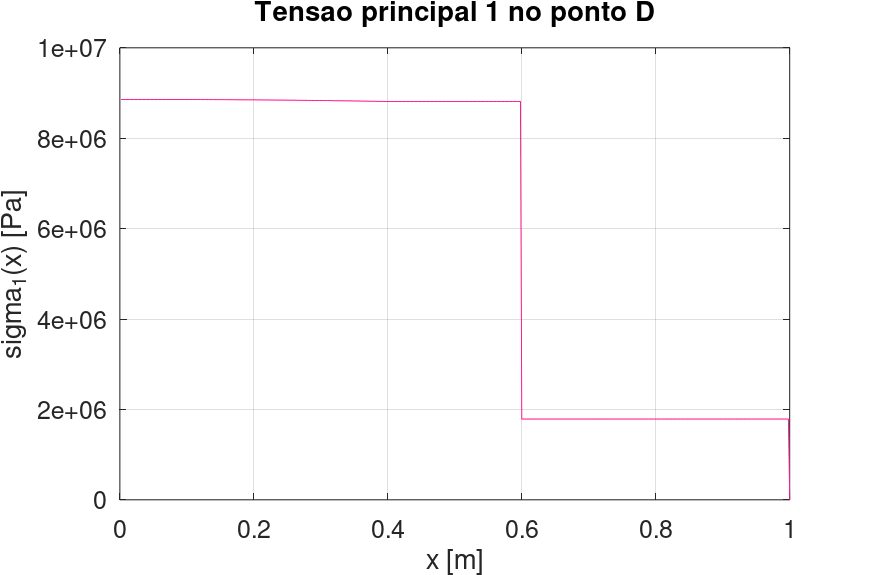
\includegraphics[scale=0.25]{figure39.png}
    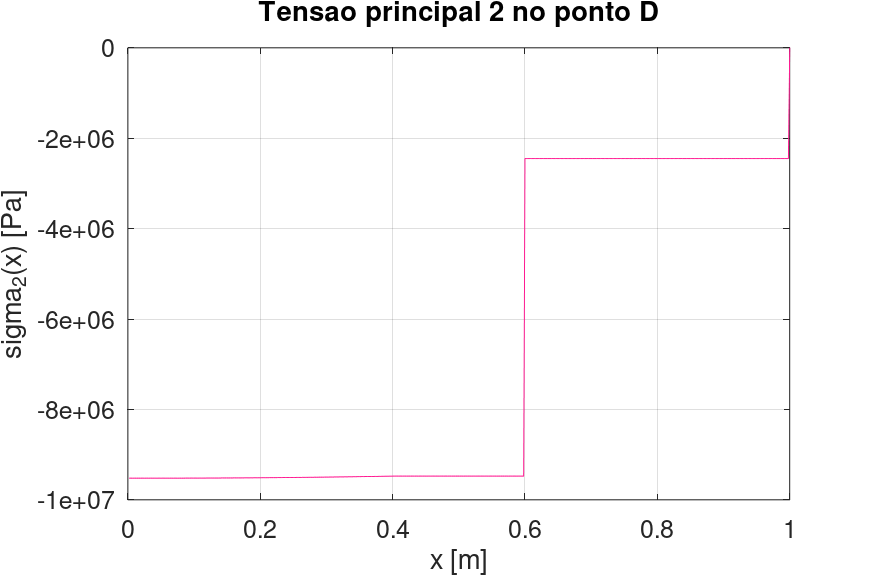
\includegraphics[scale=0.25]{figure40.png}
    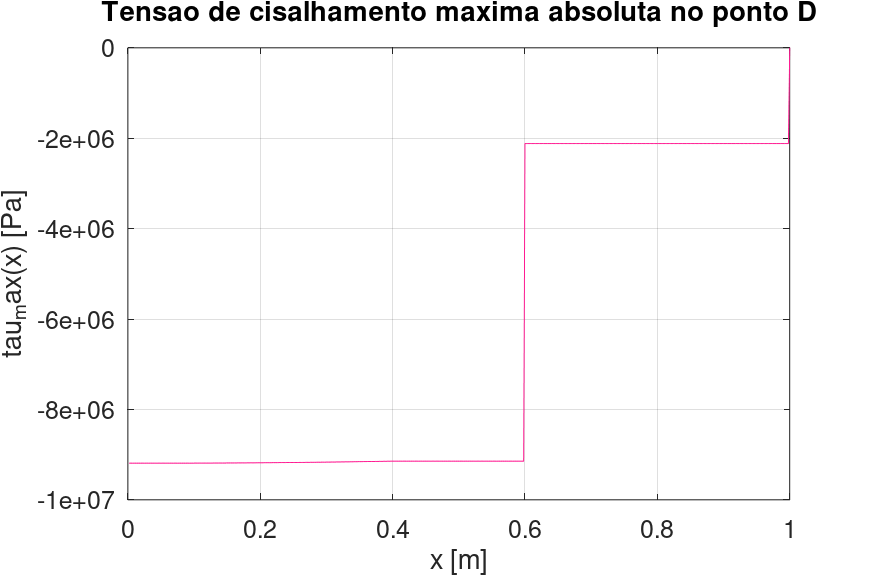
\includegraphics[scale=0.25]{figure41.png}
    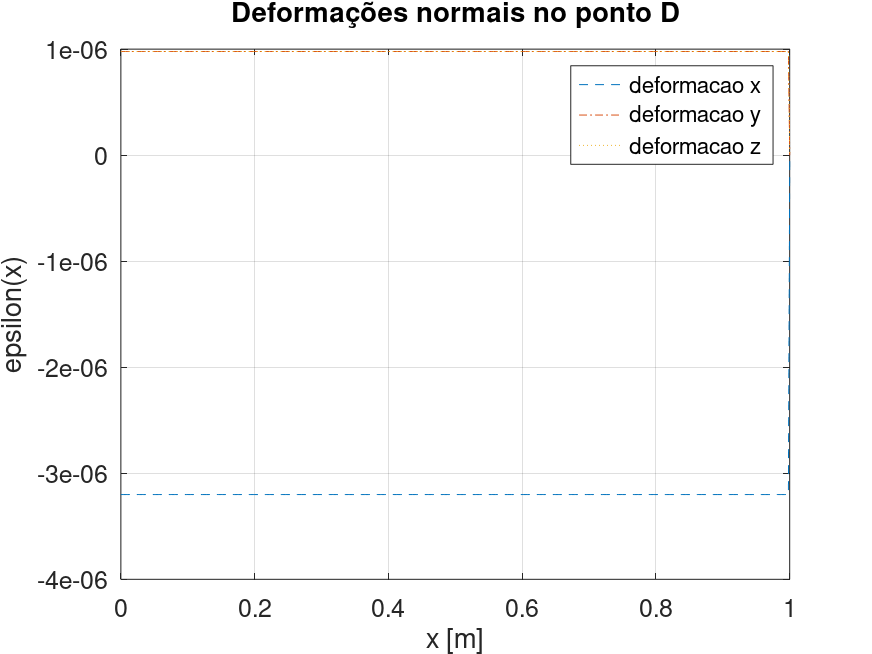
\includegraphics[scale=0.25]{figure42.png}
    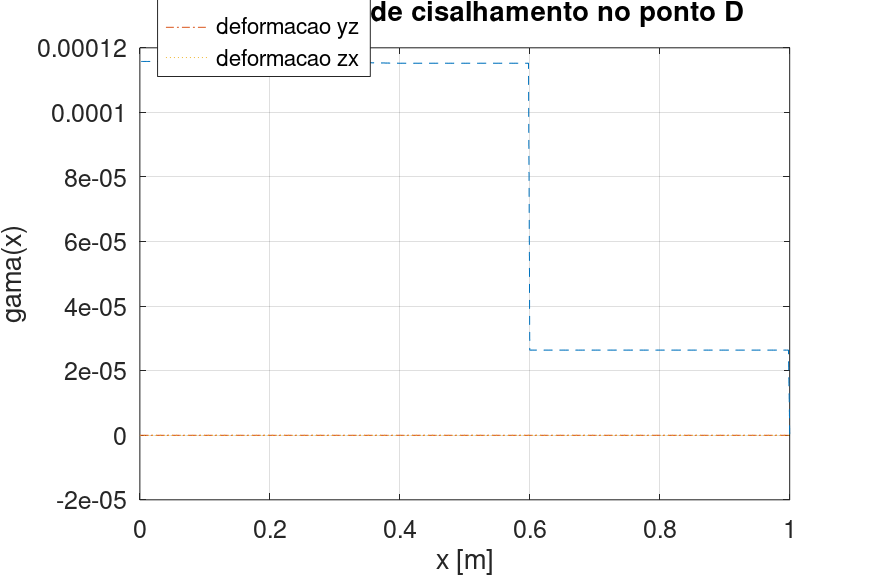
\includegraphics[scale=0.25]{figure43.png}
    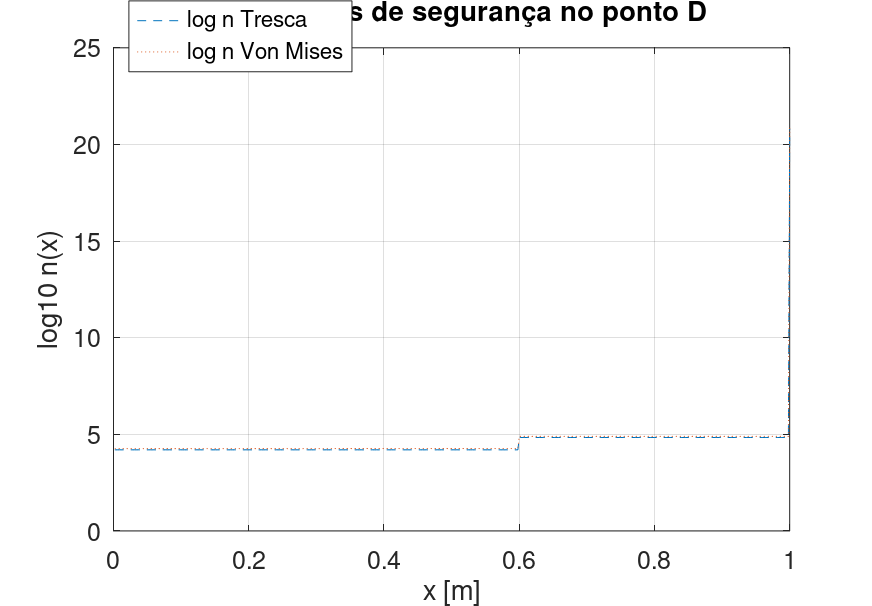
\includegraphics[scale=0.25]{figure44.png}
\end{center}

\end{document}
